%%%%%%%%%%%%%%%%%%%%%%%%%%%%%% QCD %%%%%%%%%%%%%%%%%%%%%%%%%%
\clearpage
\section{Multi-jet Validation using Data} \label{sec::BGestimation::VRQCD}
Among the ``fake'' backgrounds defined in Table \ref{tab::BGestimation::BGclass}, 
the multi-jets background including QCD di-jet and full-hadronic decays of $\vjets$ or $\ttbar$, is ignored in the estimation since it is supposed to be negligible after requiring one signal lepton and $\met>250$ in the events, based on the MC study and the past Run2 ATLAS 1-lepton analyses \cite{strong1L_3p2fb_paper}\cite{strong1L_ICHEP2016_CONF}.
However, the cross-check is always worthwhile since the impact could be fatal once it turns to contribute because of its huge cross-section. 
The other components, dominated by $W\ra\tau\nu$ and $Z\ra\nu\nu$, are estimated by the kinematical extrapolation method in which the normalization factors in Figurere \ref{fig::BGestimation::fittedSFs} are applied for $\wjets$ and top MC. Note that the normalization factors are intended to correct the mis-modeling in the hard process kinematics, but not the modeling on the fake rate of lepton candidates where MC is known to be sometimes unreliable. 
Therefore, a data-driven validation is performed in a set of specific validation regions (VR-QCD) to check those estimation. \\

VR-QCDs are defined by inverting the isolation requirement on the final state lepton with respect to the SRs, as shown in Table \ref{SRdefinition::regionDef2J} - \ref{SRdefinition::regionDef3B}. 
The abundance of ``fake'' components is enhanced by around factor of 10 with respect to the SRs, due to the high rejection factor of isolation that is typically $10-20$ ($5-10$) for fake electrons (muons). \\

Figurere \ref{fig::BGestimation::VRQCD1} - \ref{fig::BGestimation::VRQCD2} are the result for each $\meffInc$ bin of VRs-QCD. Nice agreement between the estimation and data is seen overall, implying the good MC modeling on fake lepton. Note that the multi-jets process is not included in MC thus the contribution would emerge as excess in data if it is significant, which is fortunately not the case. \\

\begin{figure}[h]
  \centering
    \subfigure[]{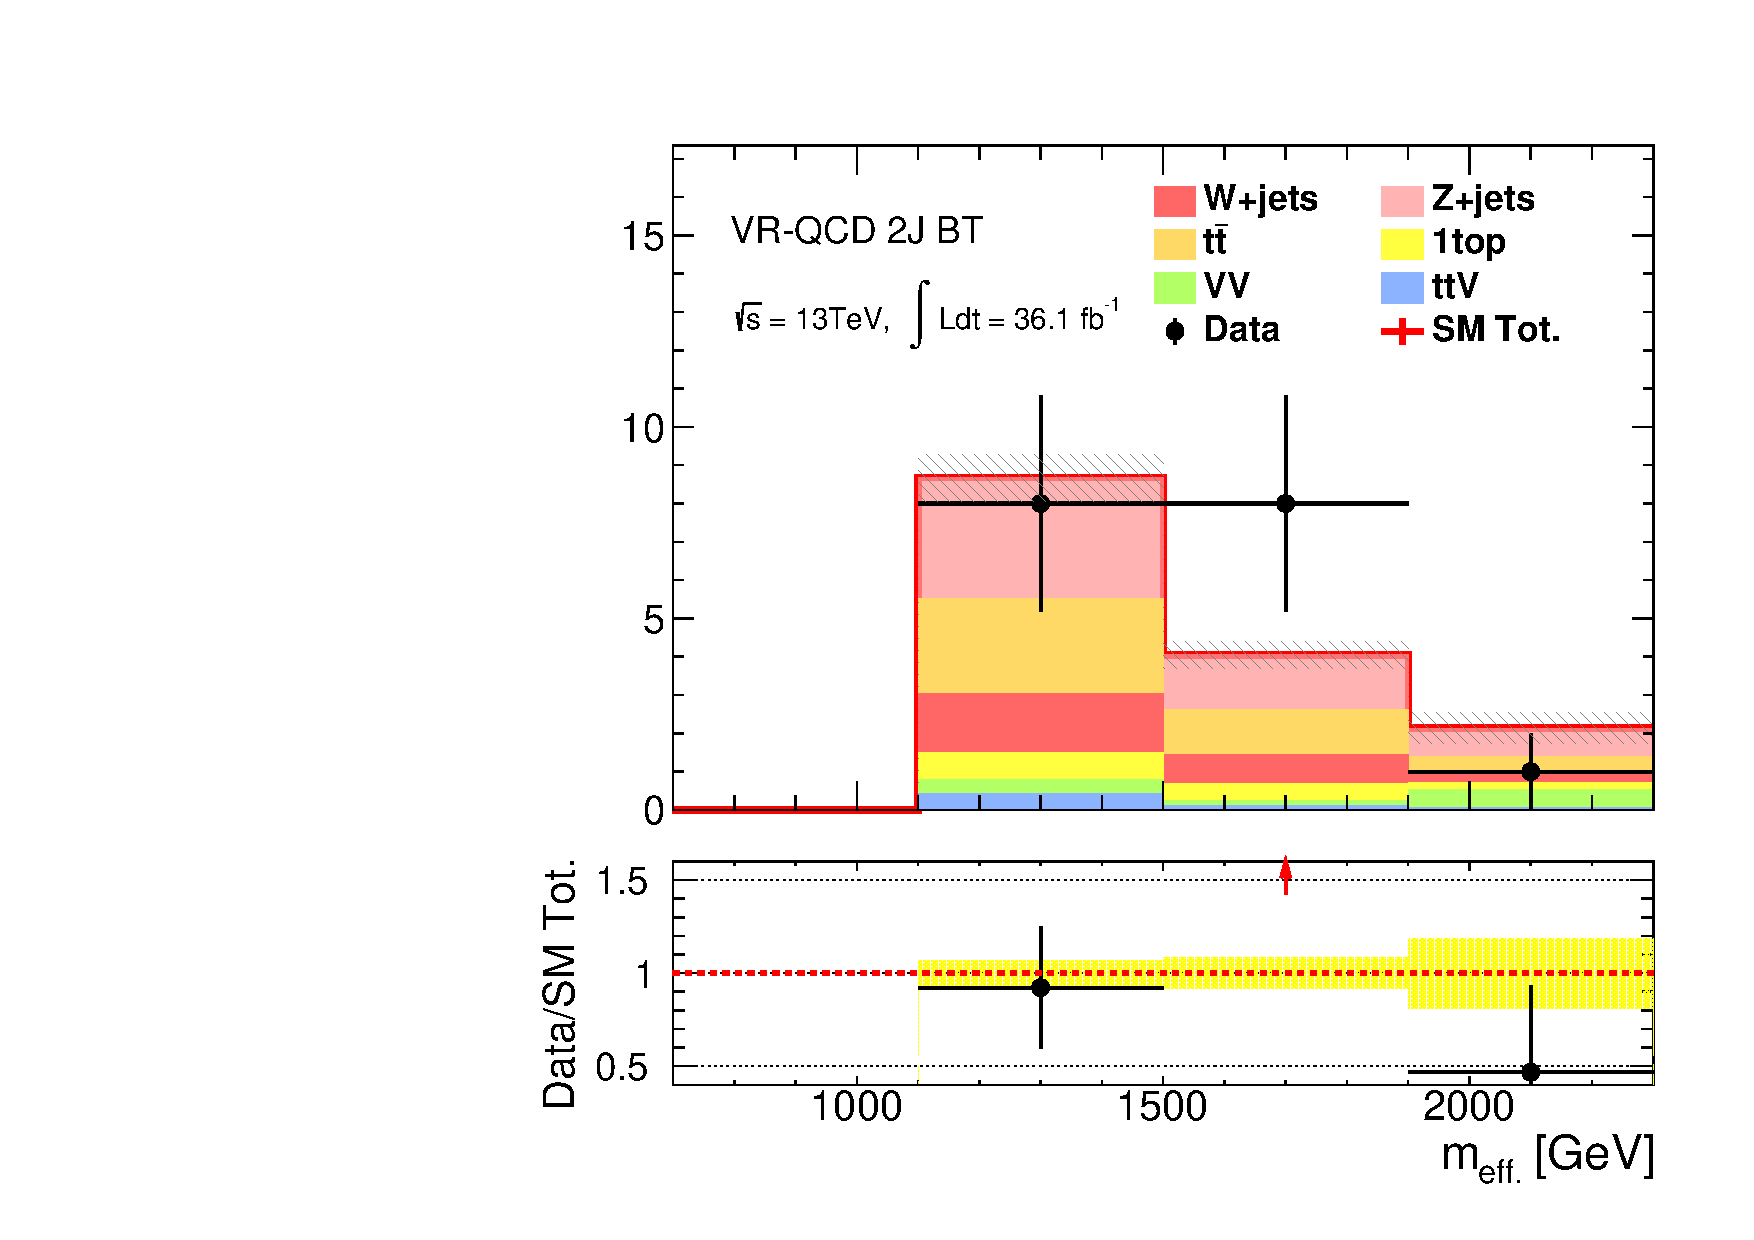
\includegraphics[width=0.48\textwidth]{figures/BGestimation/VRQCD/meffInc30__QCDCR2JMEFFInclBT.pdf}}
    \subfigure[]{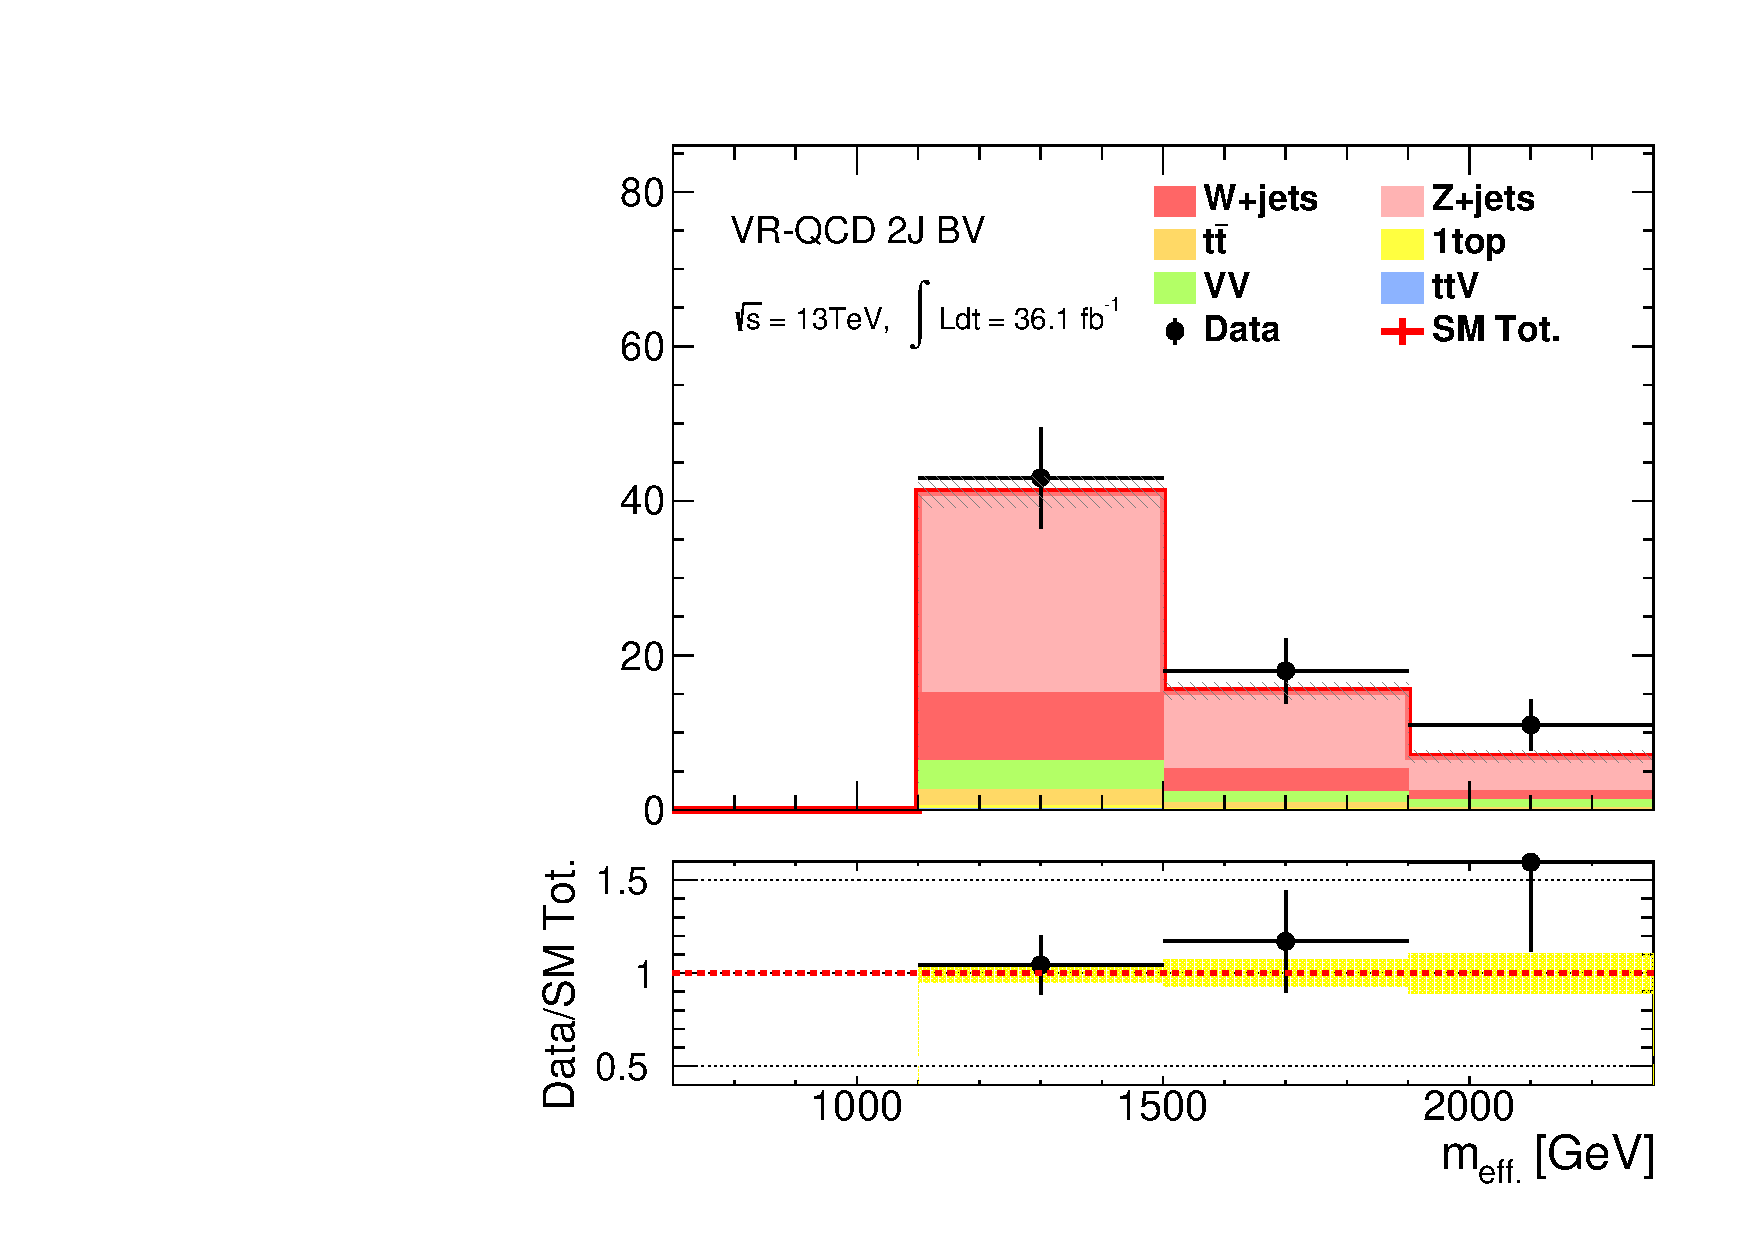
\includegraphics[width=0.48\textwidth]{figures/BGestimation/VRQCD/meffInc30__QCDCR2JMEFFInclBV.pdf}}
    \subfigure[]{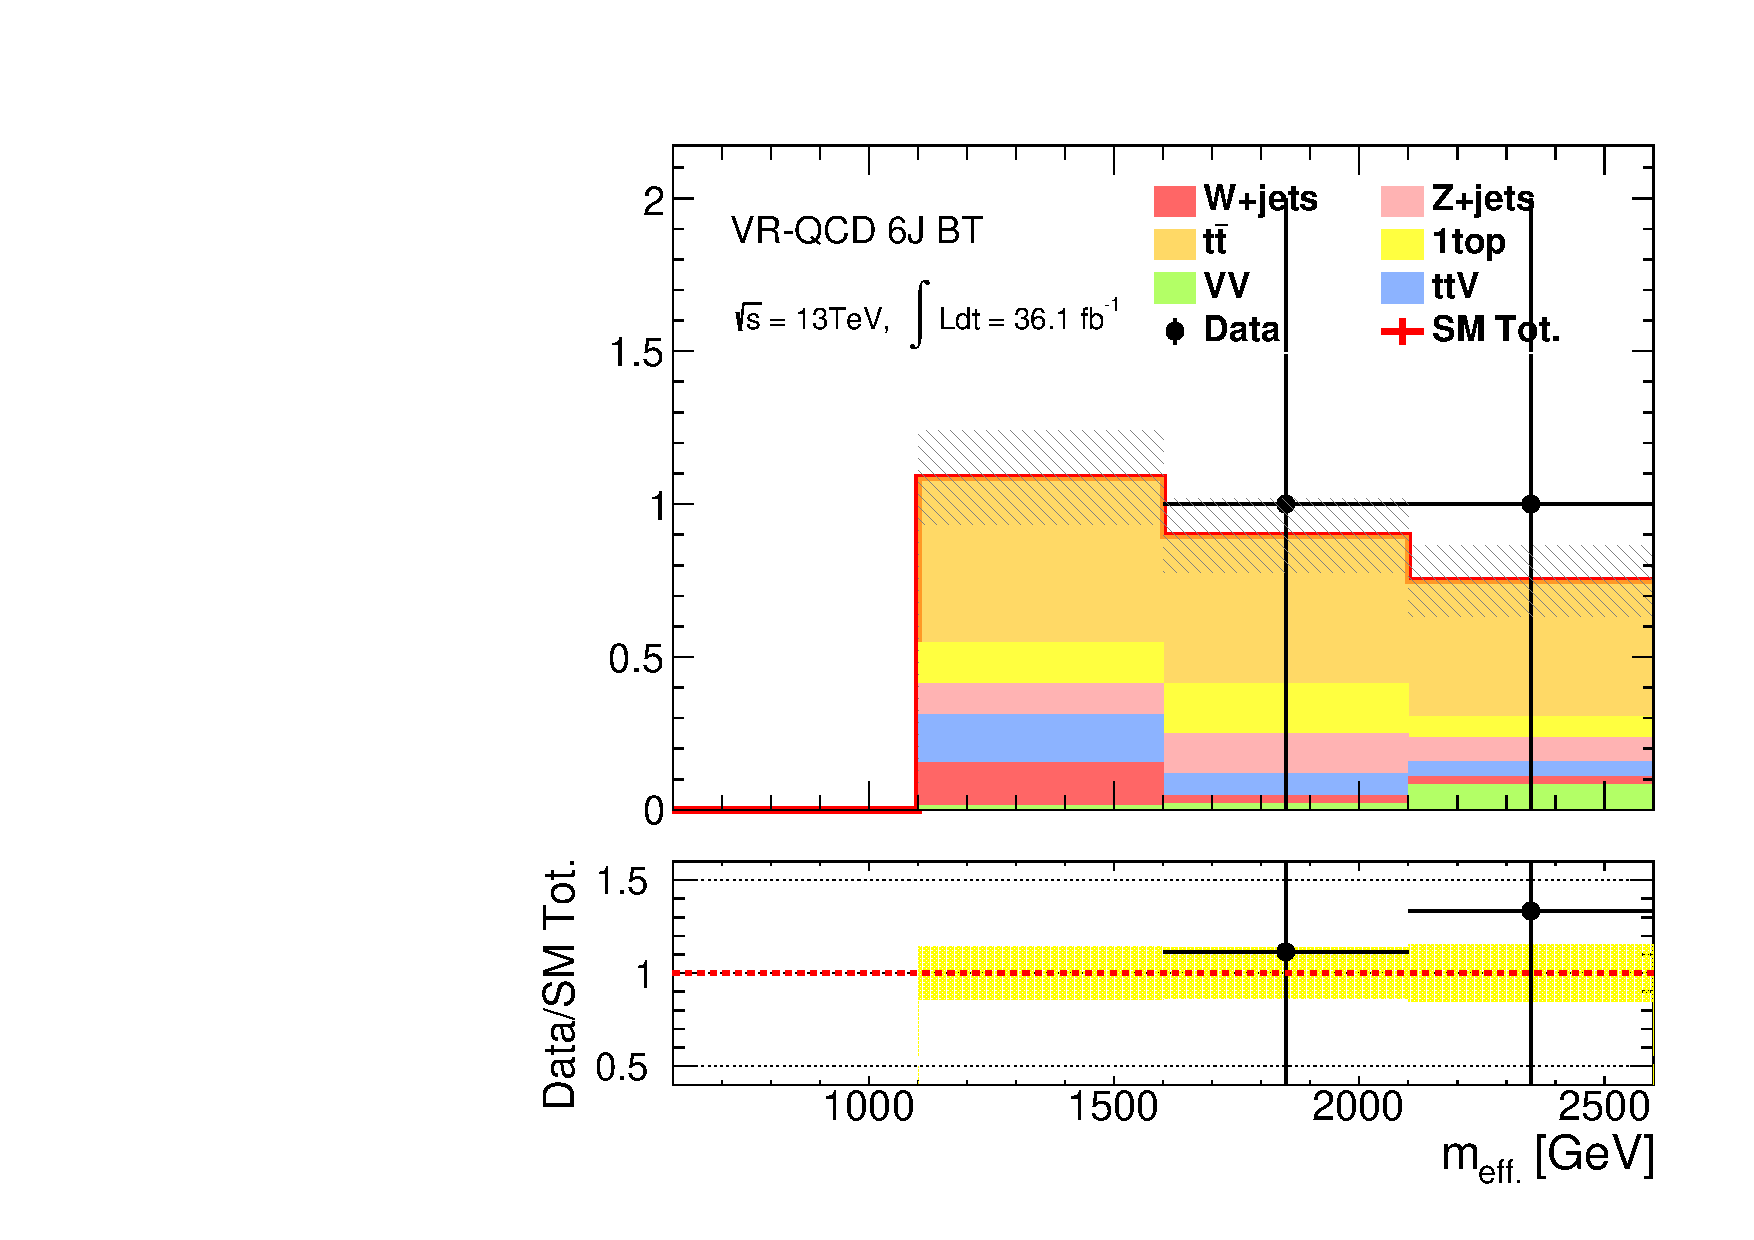
\includegraphics[width=0.48\textwidth]{figures/BGestimation/VRQCD/meffInc30__QCDCR6JMEFFInclBT.pdf}}
    \subfigure[]{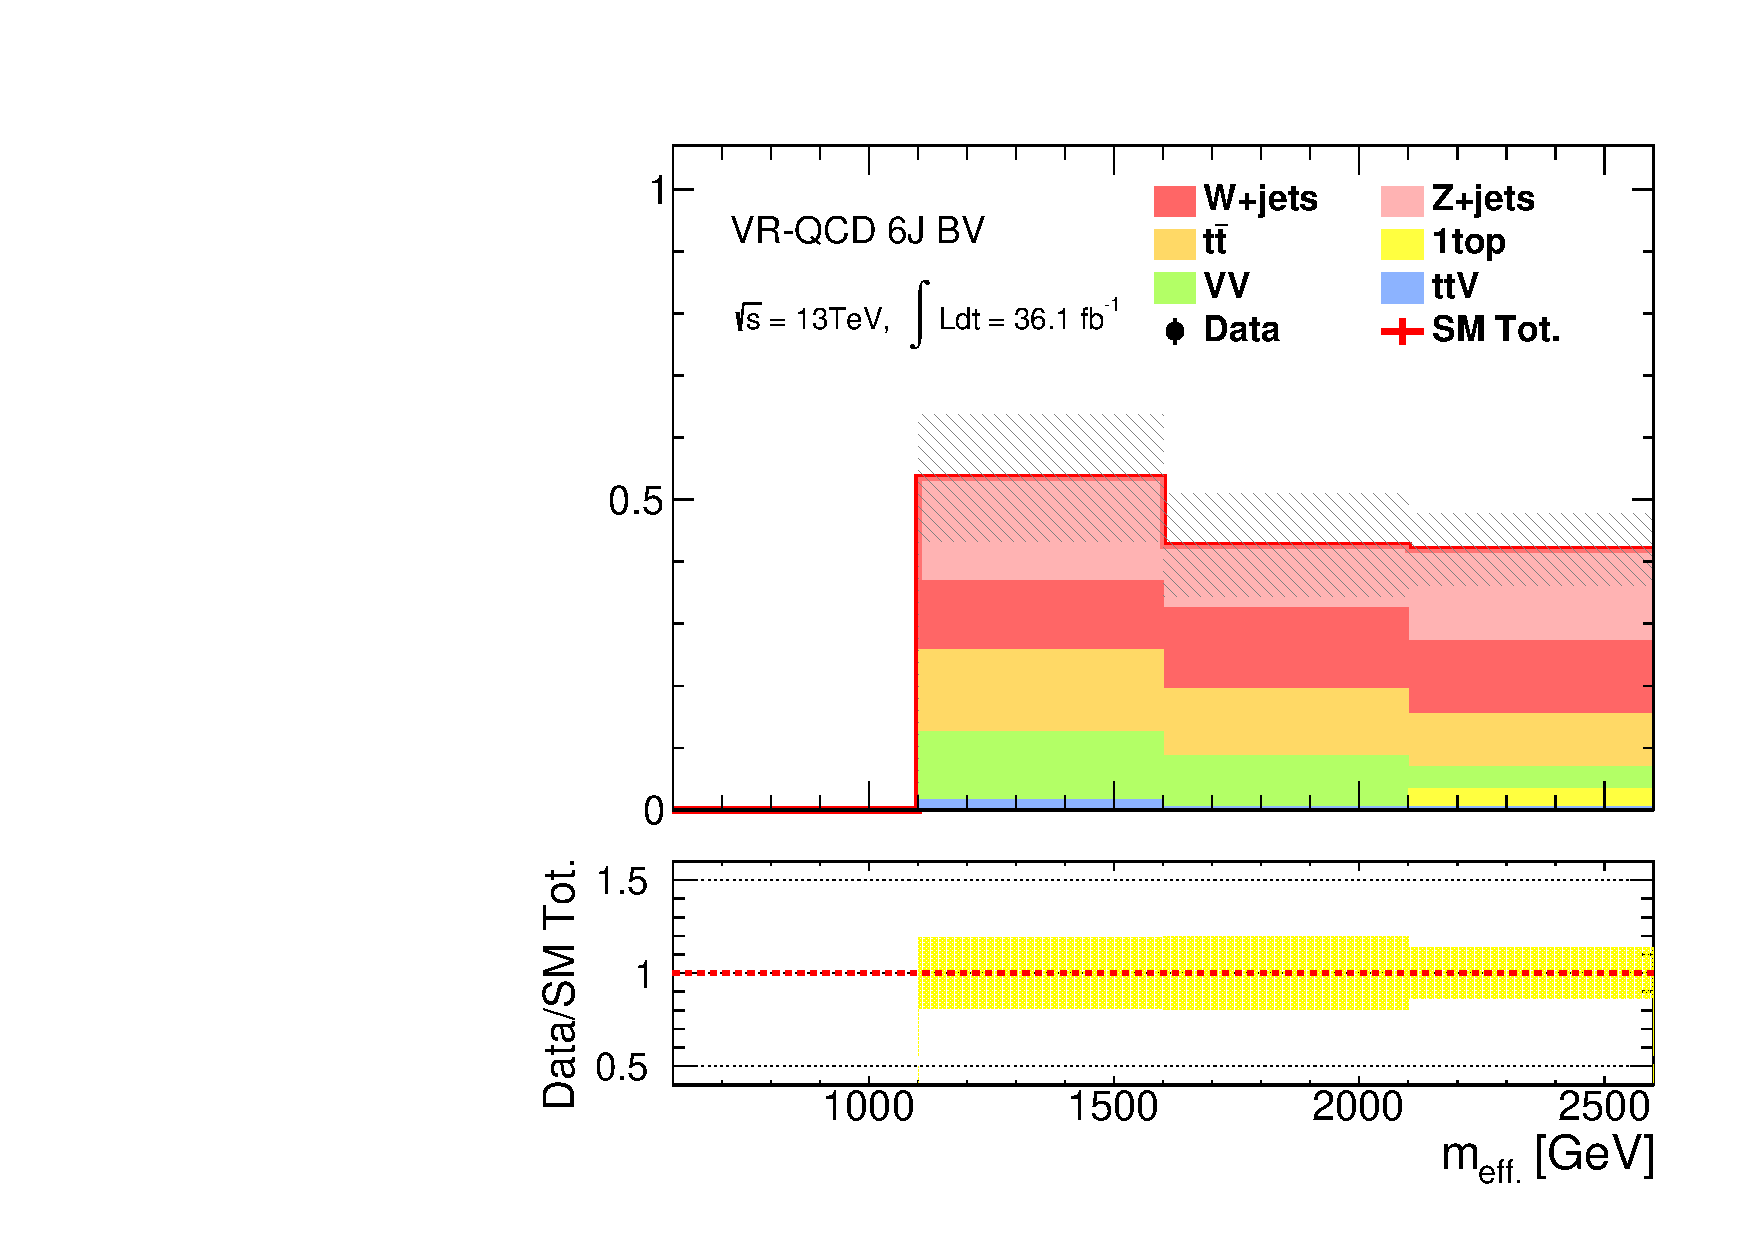
\includegraphics[width=0.48\textwidth]{figures/BGestimation/VRQCD/meffInc30__QCDCR6JMEFFInclBV.pdf}}
    \caption{ VR-QCD for towers (a) 2JBT (b) 2JBV (c) 6JBT (d) 6JBV.  \label{fig::BGestimation::VRQCD1} }
\end{figure} 


\begin{figure}[h]
  \centering
    \subfigure[]{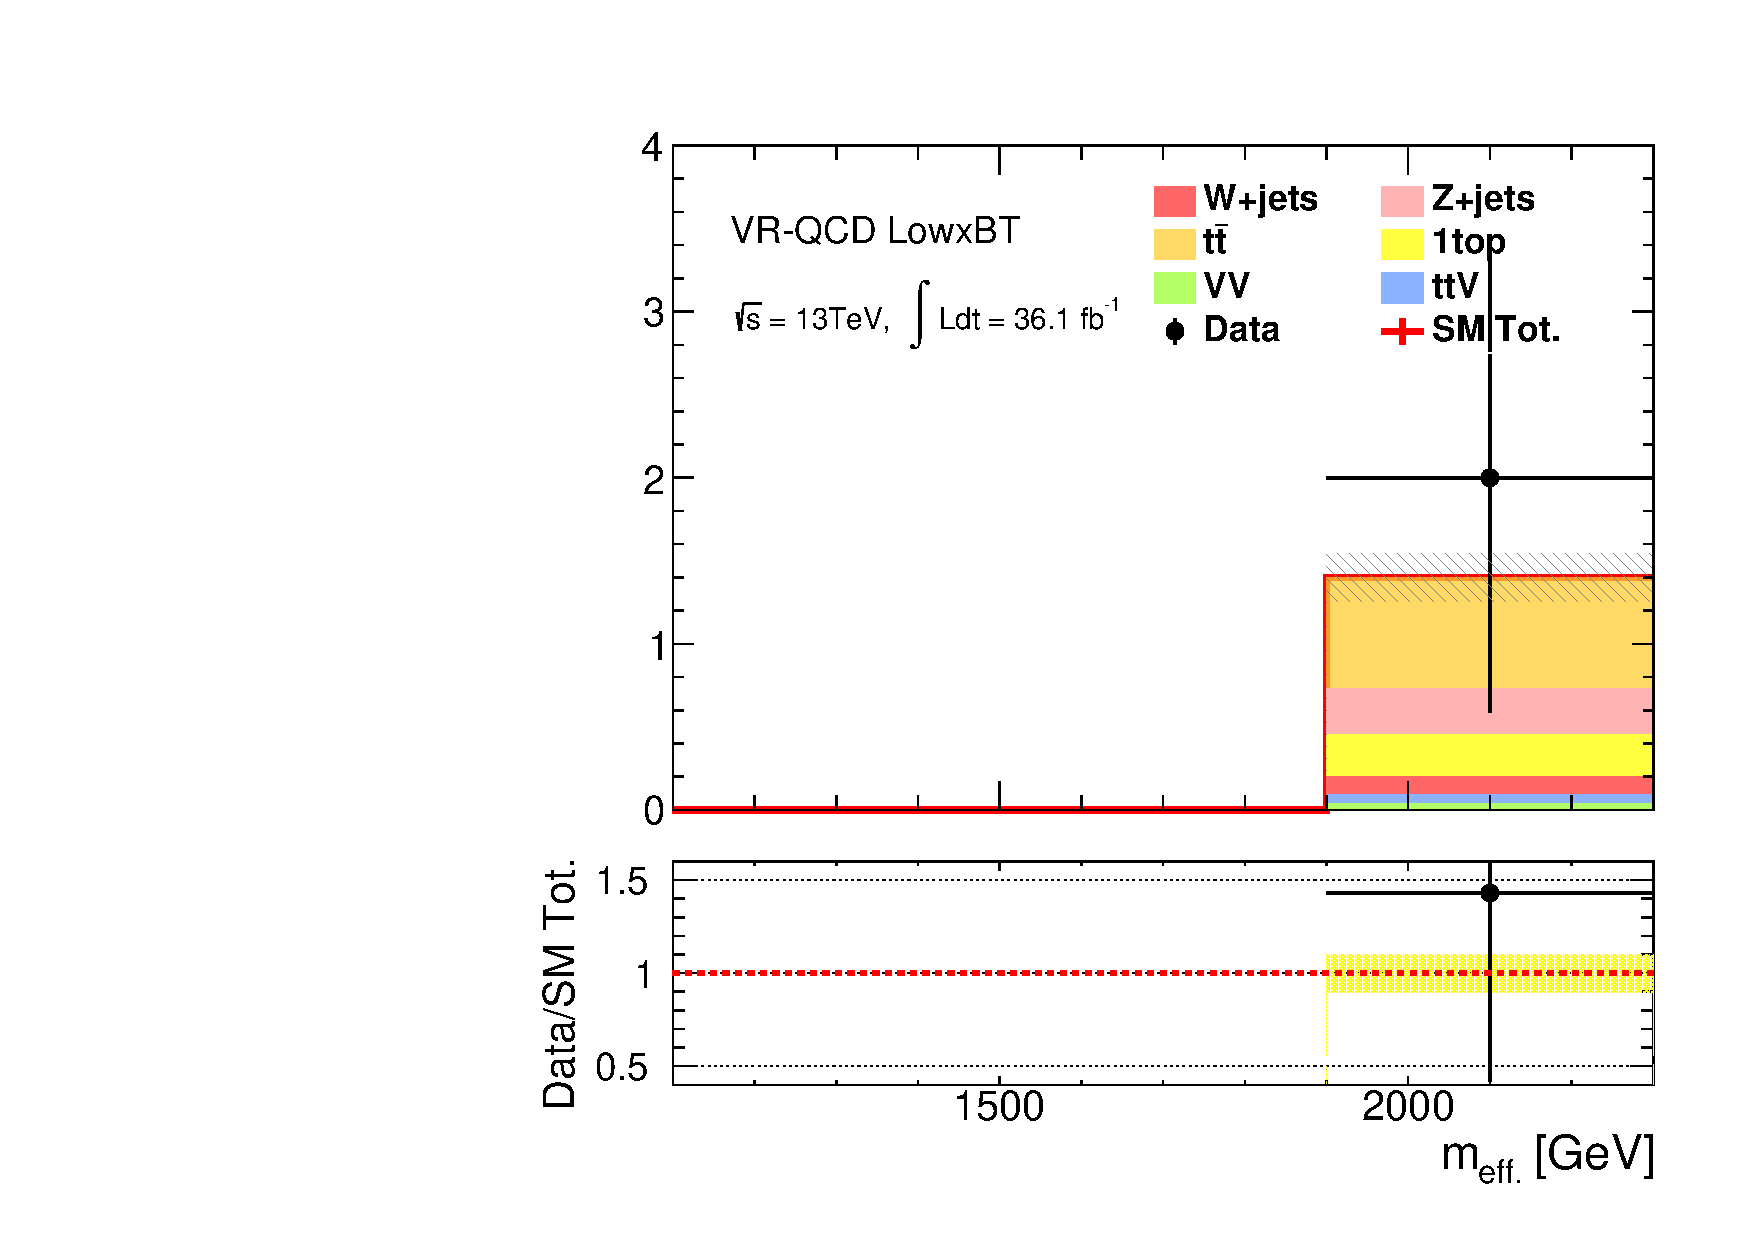
\includegraphics[width=0.4\textwidth]{figures/BGestimation/VRQCD/meffInc30__QCDCRLowxBT.pdf}}
    \subfigure[]{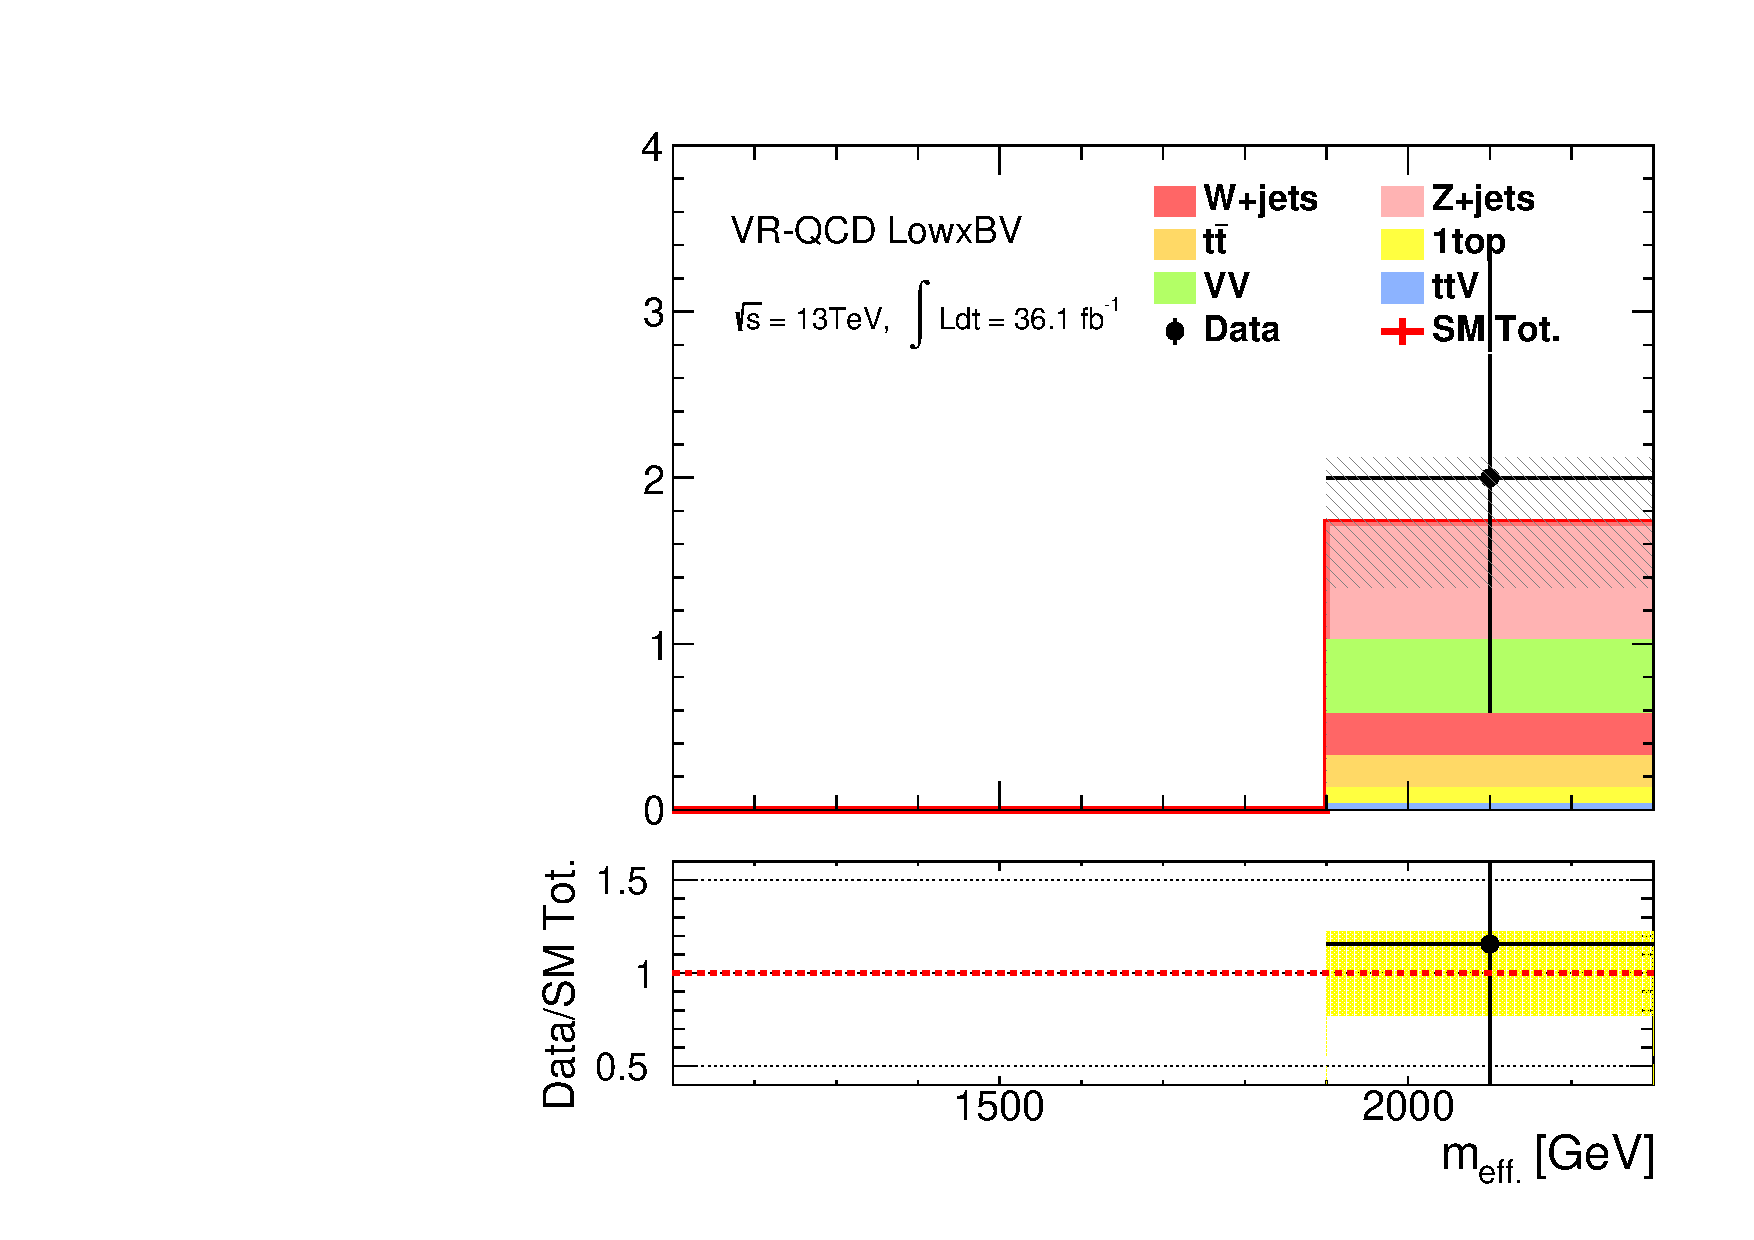
\includegraphics[width=0.4\textwidth]{figures/BGestimation/VRQCD/meffInc30__QCDCRLowxBV.pdf}}
    \subfigure[]{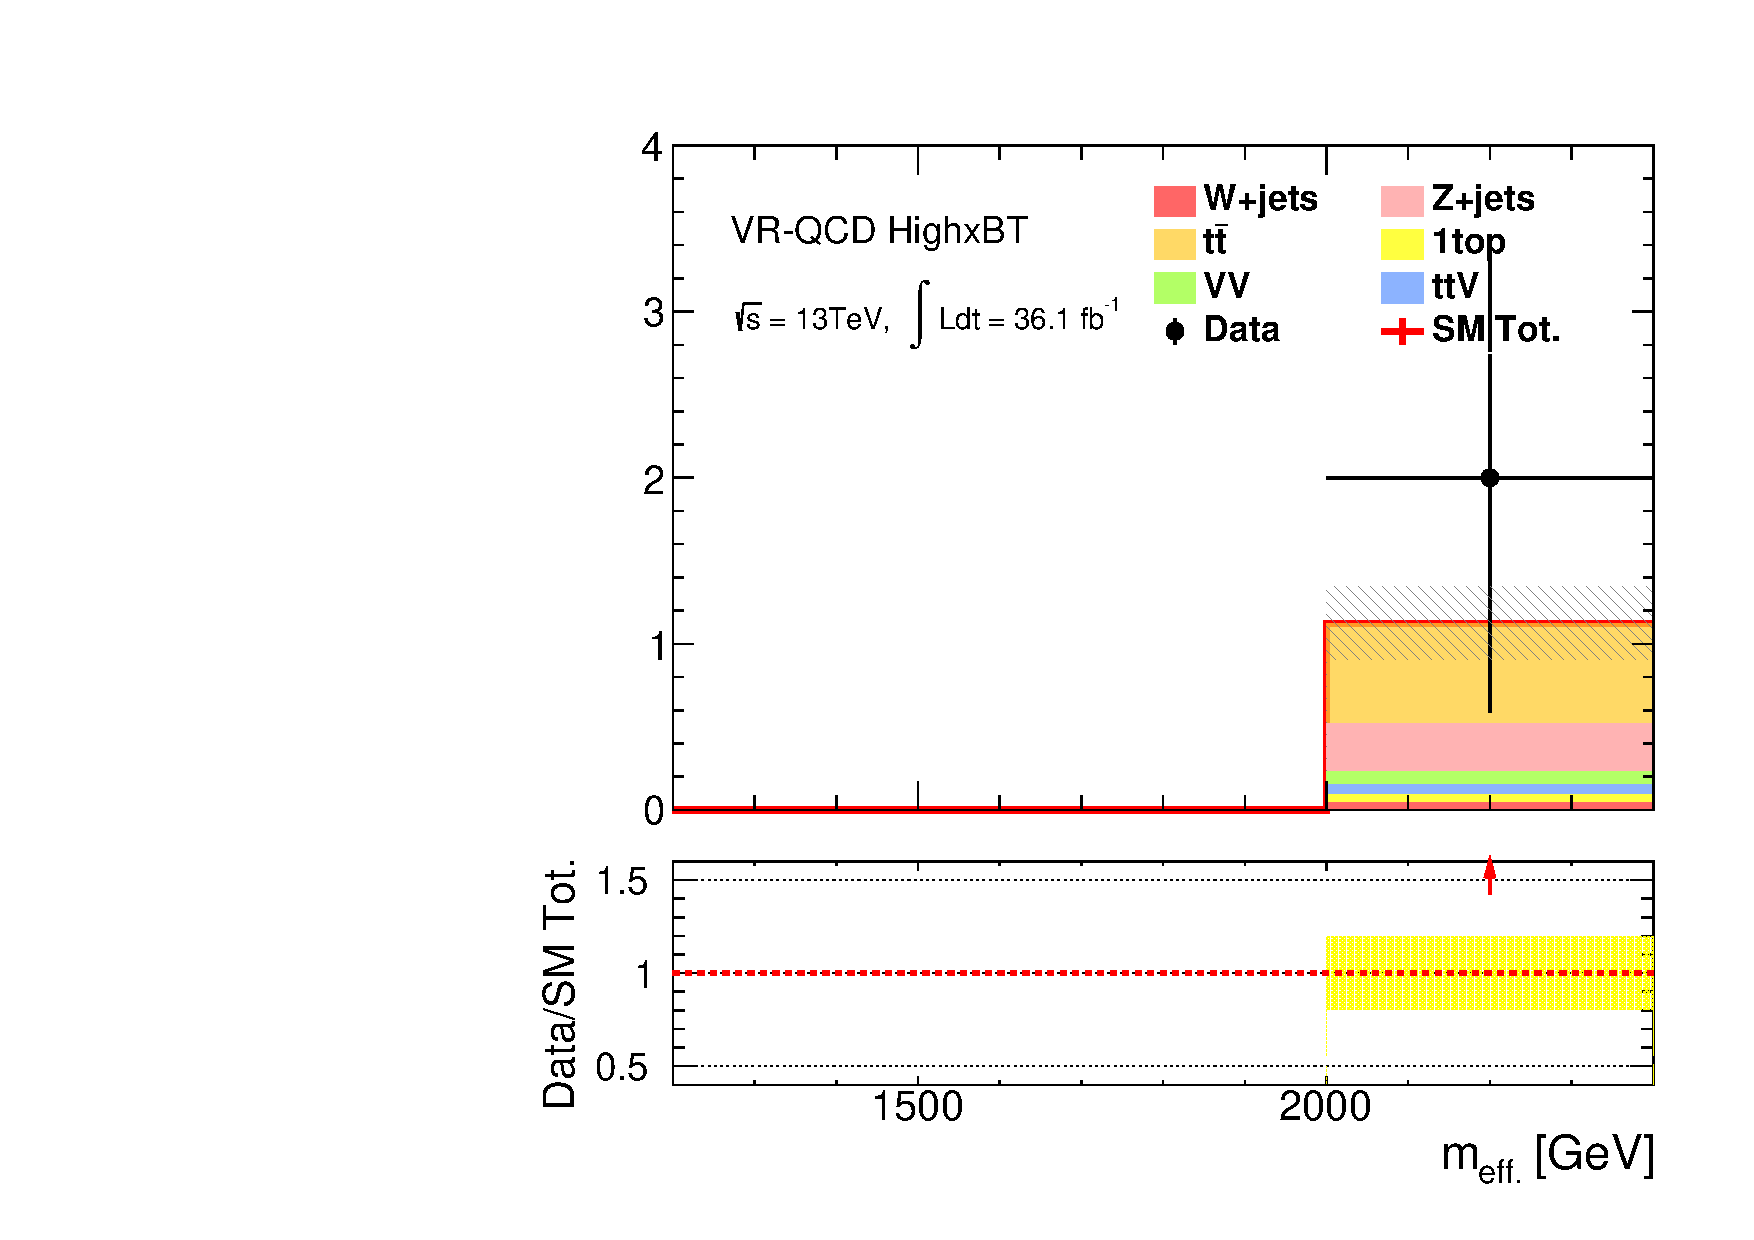
\includegraphics[width=0.4\textwidth]{figures/BGestimation/VRQCD/meffInc30__QCDCRHighxBT.pdf}}
    \subfigure[]{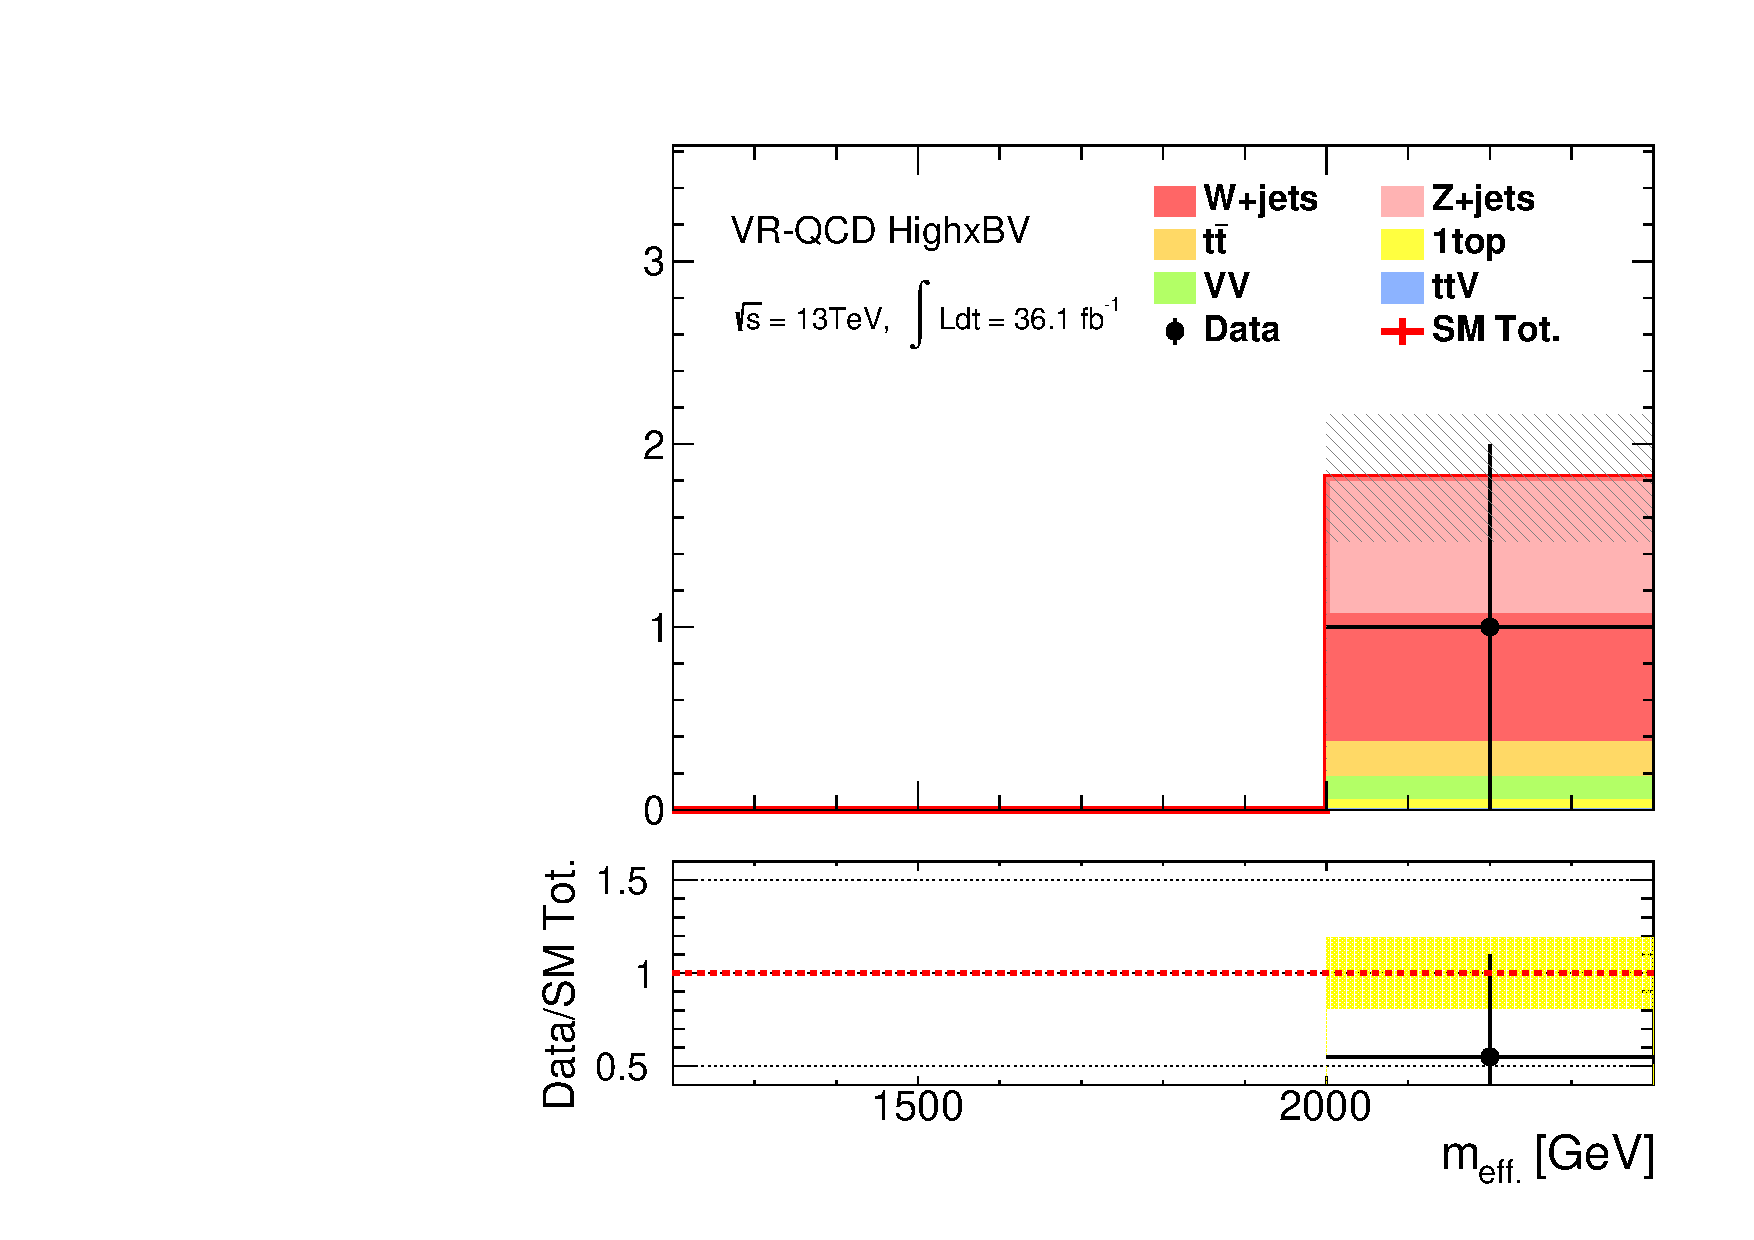
\includegraphics[width=0.4\textwidth]{figures/BGestimation/VRQCD/meffInc30__QCDCRHighxBV.pdf}}
    \subfigure[]{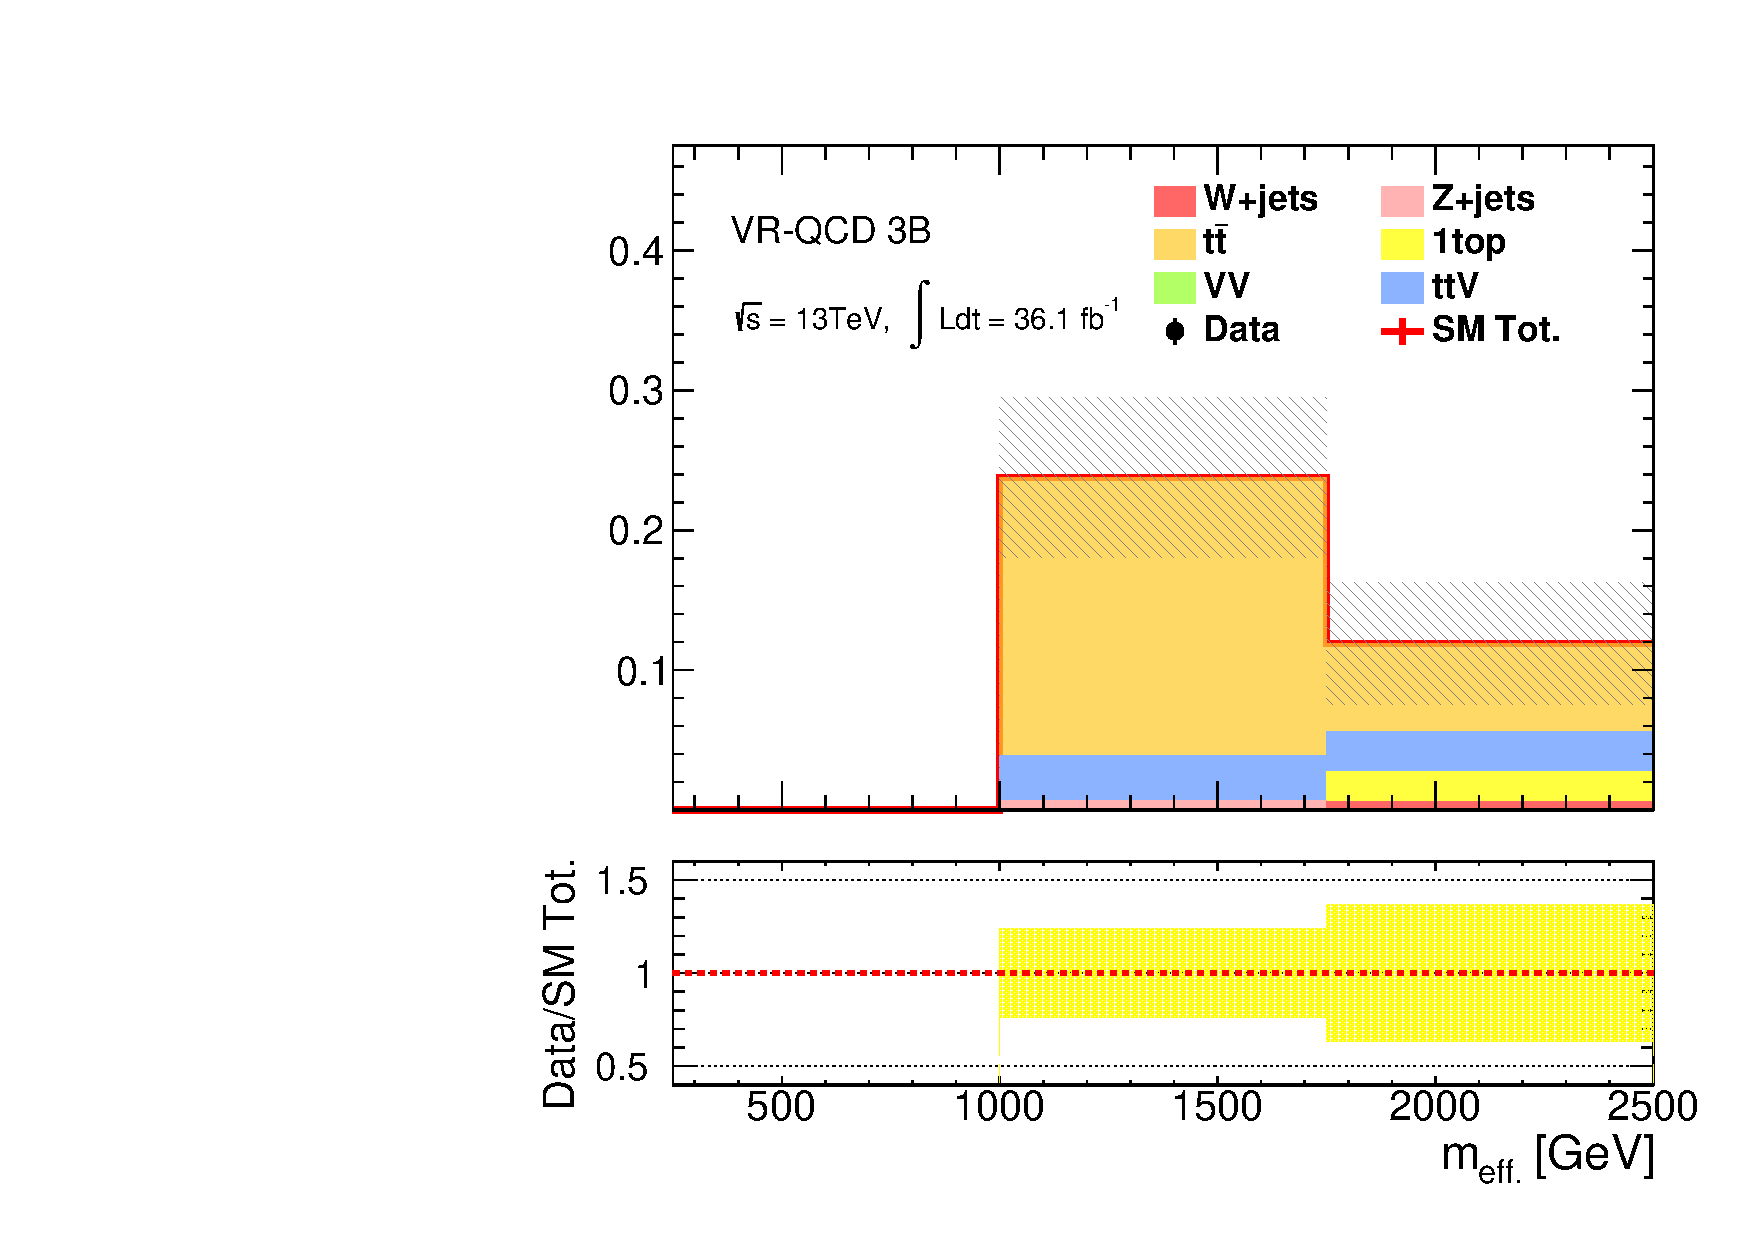
\includegraphics[width=0.4\textwidth]{figures/BGestimation/VRQCD/meffInc30__QCDCR3BMEFFIncl.pdf}}
    \caption{ VR-QCD for towers (a) LowxBT (b) LowxBV (c) HighxBT (d) HighxBV  (e) 3B.  \label{fig::BGestimation::VRQCD2} }
\end{figure} 

